\documentclass[review]{elsarticle}
\usepackage{lineno,hyperref,amsmath,adjustbox,todonotes,gensymb,float,afterpage}
\usepackage[margin=0.95in]{geometry}
\usepackage{setspace}
\usepackage[T1]{fontenc}
\bibliographystyle{elsarticle-num}
\journal{Applied Energy}
\begin{document}\begin{frontmatter}
\title{Psychrometrically characterizing the humidity and energy benefits of widening indoor set point temperatures}
\author[mysecondaryaddress]{Hongshan Guo\corref{mycorrespondingauthor}}
\author[mymainaddress,mysecondaryaddress]{Forrest Meggers}
\cortext[mycorrespondingauthor]{Corresponding author}
\ead{fmeggers@princeton.edu}
\address[mymainaddress]{School of Architecture, Princeton University, USA}
\address[mysecondaryaddress]{Andlinger Center for Energy and the Environment, Princeton University, USA.}
\begin{abstract}
Among other approaches of reducing building-related energy usage, modifying the indoor air temperature set points has been proven a very efffective approach. Building on recent findings that expanding the range of set points can achieve the same level of occupant comfort while achieving energy savings, we want to investigate the possibilities of pushing the set point ranges further in this study. To achieve the further expanded indoor air temperature set point yet still addressing the heating/cooling loads, we assumed the usage of supplemental radiant heating and cooling systems in average household across the continental US. Interpolating the psychrometric processes across the weather data we collected, we were able to show the importance of having humidifiers for all-air systems through a spatial analysis. Our analysis also showed that more than 60\% of the dehumidification energy demand can be mitigated from a higher set point during the cooling season. These results are helpful to illustrate the inherent strength of radiant systems when addressing latent demands in the indoor environments. Further investigations on how different occupancy schedule and occupant density may be helpful in advancing our understanding on the latent-load-mitigation capability of radiant systems.
\end{abstract}
\begin{keyword}relative humidity\sep radiant heating and https://www.overleaf.com/project/5e41b797fc7edc000135b473cooling\sep cooling degree days\sep latent loads\end{keyword}\end{frontmatter}
\tableofcontents
\section{Introduction}
% Energy savings of alternative energy systems/delivery systems.

%Why radiant
As there are many different types of heating and cooling systems that are widely available, we want to investigate particularly the implications of radiant systems in contrast to all-air systems since the contrast would be larger. This is because the radiant systems do not need to explicitly condition the air temperature, which will result in smaller heating and cooling load since water and other working fluids are better heat carriers. In the meantime, radiant systems appear to have comparable if not better thermal comfort implications according to existing studies, hence forming good comparison to the prevailing air-based heating/cooling systems in the US.

%The relationship to relative humidity.
Unlike air temperature, or the targeted fluid/surface temperature that are often used in the control of air or radiant systems, relative humidity (RH) is a much less commonly observed control variable. Relative-humidity-based control is currently used in more strictly-controlled environments such as piano rooms, archival storage rooms and specialized medical facilities. RH-based control is currently very expensive for residential or large commercial projects to consider. This is not only because the demand of RH-specific environments is less common, but also because the value of RH is codependent on the condition of the moist air condition, and cannot be easily controlled through a feedback control loop. 

%Air as we know it
The moist air in a room is a mixture of both dry air and water vapor. Dry air has properties that are very close to ideal gas while the water vapor is ideal gas, we model their mixture using the ideal gas law and can estimate this mixture’s remaining properties (pressure, humidity ratio and enthalpy) when a specific set of property (temperature and RH, in this example) is given. Graphically, this is also often explained by the psychrometric chart published by ASHRAE. However, the actual psychrometric processes that air conditioners undergoes is a myth to most users, since the feedback variable that most of their systems would allow them to control is only the air temperature. Although ASHRAE does recommend RH to be maintained between 30\% to 60\%, adding humidity to the air is still a secondary concern when people are purchasing and installing home air conditioning systems. 

%RH – dry and wet
According to some latest research, the health implications of RH can be significant, although often in a delayed and indirect manner. Reports on RH below 20\% could cause eye irritation and dryness/stuffiness complaints, and ultra-low RHs below that may even cause eye and air pathway and skin symptoms. RH below 10\% could even desiccate the mucous membrane over time and lead to further agitation with both the eye and nasal cavity. Conversely, higher RH levels also have the potential to deteriorate building materials and grow mold that may lead to respiratory symptoms among building occupants. However, the RH that would allow rapid growth of bacteria and viruses are often found to be at least 75\%, which is much higher than the mandate from ASHRAE or ISO 7730 (30\% to 70\%). There is, ultimately, very little regulation or guidelines regarding what the RH inside a room should be kept at, and anything above 30\% and below 60\% is acceptable. This is potentially also the reason why RH is much less controlled in conventional systems.

%Relationship to Energy
Existing literature have already established the link between energy savings and expanded set points of air. The verified energy potentials were demonstrated through air-based systems in simulated building cases through different climates. This included both the sensible and latent heat following the underlying hypothesis of the building case used and the occupancy density that was selected. Using radiant systems may prevent the excessive energy usage needed to remove the latent heat in the air in the summer. The relationship between the sensible and latent cooling load is less often studied but has seen some recent advances: new concepts such as the enthalpy degree days and latent enthalpy days were proposed in contrast to the cooling degree day method used in estimating annual cooling loads.

%What we want to do with this study  
In this study, we hope to take advantage of the existing literature to understand the benefit of further expanding the set point temperatures through the usage of radiant systems. This would include discussions on the energy savings from preventing the latent loads that would otherwise have occurred when using all-air systems, as well as the improvement of RH without additional humidifiers for the heating season.  To better illustrate the energy saving potentials and the corresponding improvement in RH, we will run the analysis through hypothetical household located across the 48 continental states in the US to illustrate the energy and humidity potentials that can be found across different areas. 

\section{Methodology}
    % \subsection{Base Assumptions}
    %     Hoping to create a generic building energy footprint for comparison across the United States, we are assuming an average household with average square footage, household member counts, and energy consumption profiles that are made publicly available by the Department of Energy and US Census. For the purpose of this study, we consider only the residential conditioning systems. For this purpose, we assume the size of the household to be 2.52 occupants (cite US. Census.), which requires no more than 37.8 CFM of fresh air according to ASHRAE. In order to estimate the required fresh air rate, we assume the size of the house through the average size of buildings built (cite DOE?) as 2392 squared feet. As according to ASHRAE Standard 62, the newly-built buildings are instructed to achieve an infiltration rate of 2 CFM per every 100 squared feet, this allows us to estimate the ventilation rate of the hypothetical average house to have 47.84 CFM through infiltration. This is above the required fresh air amount for 2.52 hypothetical occupants in the average household in the United States. Assuming the height of the houses to be 9 feet, we obtained a fresh air percentage of 18 per cent, which allowed us to estimate the condition of the mixed air with a targeted indoor air condition and outdoor air condition.  The set points and the psychrometric processes we are assuming are introduced separated in the subsequent sections.

    
    \subsection{Cooling, Heating and Enthalpy Degree Days}
        Degree Day (DD) is a method that ASHRAE currently still recommend using when measuring how outdoor air temperature variation may impact the energy use. It compares the outdoor temperature to a defined base temperature, which is naturally a temperature-based method used to explain building energy consumption. As we are attempting to illustrate the differences between the radiant and air-based differences, DD is an apparent choice that circumvents the selection of more explicit building systems. In degree-day theory, the base temperature separates times where buildings need conditioning from times it does not. This applies to both the heating and the cooling case, or otherwise known as cooling degree day (CDD) and heating degree day (HDD) methods. (Use equations for both here).  The base case can often be considered the equivalent of set-point temperature, and is recommended to be set at 18.3 C(65 F) by ASHRAE.

However, as both the CDD and HDD method are based solely on the outdoor dry-bulb temperature, the latent loads are apparently overlooked. This is particularly true for the cooling scenario. Researchers have proposed alternative such as the enthalpy degree days (EDD), where the enthalpy of the air of the day can be compared to the base case enthalpy. Huang et al. first suggested the possibility of estimating the latent loads through a concept known as latent enthalpy degree day, while Krese et al. further perfected it by suggesting the EDD approach in 2012 through 2013. This is further assessed in a more recent research by Jimeno and Schulter where they proposed a Degree of Enthalpy Gradient, or DEG. It is a new advancement in the direction of assessing the latent load in buildings by combining the heating and the cooling demands and creates extra difficulty in analyzing the cooling and heating cases independently for us. 

The heating and cooling season is done with the building systems. 

\subsubsection{Cooling Processes}
    For the cooling scenario, conventional air handling units uses evaporative cooling to cool the outdoor air down to set point per the design of the cooling system. This process can be simplified on the psychrometric chart as the air temperature from the outdoor condition being cooled down to the set point at the desired indoor condition. Previous study has demonstrated the clear energy benefit of expanding the set points, yet had yet to unravel the latent energy benefit caused by the changes in set point temperature.

    \begin{figure}[h!]
    \centering
    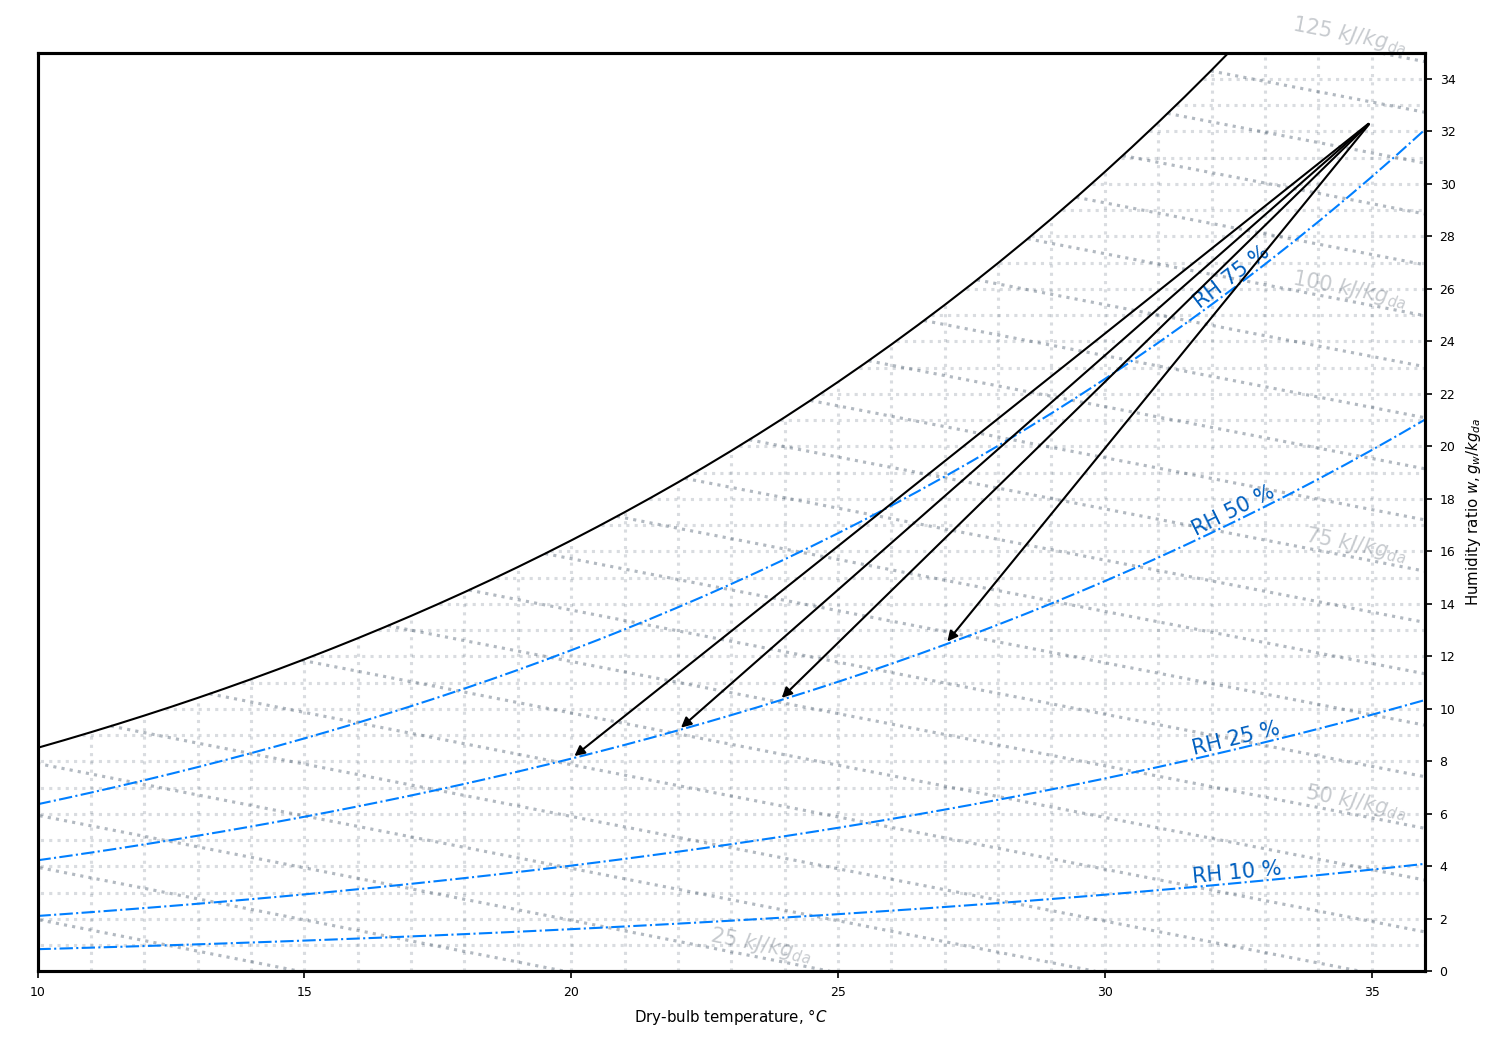
\includegraphics[width=\textwidth]{coolingcases.png}
    \caption{Example psychrometric processes under different set points for the cooling scenario.}\label{fg:cool}
    \end{figure}


    %This is how we calculate the changes in enthalpy against CDD. 
    We want to compare the impacts of having different set points specifically focusing on the differences in latent loads, which we are showing in the psychrometric process in the figure above. While maintaining the same level of desired RH, the changes in the energy demand is not fully reflected by the changes in dry bulb air temperature. We can explicitly compare the overall (latent and sensible) and sensible load by comparing the cooling degree days and the enthalpy degree days of identified set points for the cooling season and the outdoor temperature. 

    %Psychrometrically
    Psychrometrically speaking, this process is shown in Figure~\ref{fg:cool}, when air is cooled from the outdoor conditon with high dry-bulb temperature and relative humidity, eventuallly reaching the four different set points at the same desired level of RH: 50\%. The differences between the end-state enthalpy can be easily characterized by $\Delta h$ for the different set points and the outdoor temperature. We will compare this with the resulting hourly cooling degree days of each specific weather file. Following the definition of CDD by ASHRAE, we calculate the cooling degree days with Equation~\ref{eq:CDD}. Here, the cooling degree days for a defined reference temperature is $CDD_{t_{bal}}$ for a specific defined reference temperature $t_{bal}$. The rest of the parameters here are $n$ as the number of days over the desired period, and $\bar t_{o,i}$ as the daily average outdoor temperature ($\degree C$). For our purpose of the analysis, to analyze the different set points of the indoor air condition, we will use four different $t_{bal}$ values.     The ASHRAE recommended set point range is 74$\degree F$to 80$\degree F$in the summer, while a typical radiant cooled space will use 75$\degree F$(24$\degree C$) air temperature with no greater than 50\% RH, which is the equivalent of a lower dew point temperature (approx. 12.2$\degree C$) to avoid condensation.  The lowest will therefore be 18.3 $\degree C$ as suggested by ASHRAE for CDD calculation, with two extra data points as suggested by ASHRAE to be 23.3 $\degree C$ (74 $\degree F$) as well as 26.67 $\degree C$(or 80 $\degree F$, as recommended set point by ASHRAE) and up to 28 $\degree C$ (Sui \& Zhang, 2015) for the indoor air temperature in radiantly cooled environment. 

    \begin{equation}
    CDD_{t_{bal}} = \sum_{i=1}^n (\bar t_{o,i}-t_{bal})^{+}\label{eq:CDD}
    \end{equation} 

    To characterize the variations of the latent loads relating to only the enthalpy differences, the same set of dry bulb temperatures are used, while the enthalpy degree days are calculated similarly using Equation~\ref{eq:EDD}. Here, we characterize the total enthalpy differences between the state of the outdoor air ($\bar h_{o,i}$) that needs to be conditioned to a specific set point with enthalpy ($h_{bal}$). 

    \begin{equation}
    EDD = \sum^n_{i=1}(\bar h_{o,i}-h_{bal})\label{eq:EDD}
    \end{equation}

    To compare the sensible with the latent demand, the output from Equation~\ref{eq:CDD} (in Kelvin) needs to be compared with the output from Equation~\ref{eq:EDD} (kJ/kg of dry air). To achieve the same resulting unit, we will be multiplying the CDD values with the equation to calculate $c_p$ with Equation~\ref{eq:cp}, where the specific heat ($kJ/kg\cdot K$) can be calculated with a given  humidity ratio $w$. Multiplying CDD obtained through Equation~\ref{eq:CDD} with corresponding $c_p$, we may therefore obtain a specific enthalpy of dry air that is comparable to specific enthalpy of moist air obtained via Equatino~\ref{eq:EDD}/

    \begin{equation}
    c_p = 1.005 + 1.884 w \label{eq:cp}
    \end{equation}
    %This is actually the discussion of system sizing, which should go either to conclusion or discussion... Can expand to - what's going to happen when we simply change the set points in systems? 
    This calculation is aimed at emphasizing the amount of additional cooling needed when the feedback control variable is only dry bulb air temperature instead of both air and relative humidity. As is highlighted with green in the graph we generated, assuming the same amount of cooling capability but targeting only the dry bulb temperature instead of air mixture at different set points, the sizing  

\subsubsection{Heating Processes}
    %RH difference - map
    For the heating scenario, we will be operating under two stages of hypothesis. The first hypothesis we want to examine is there being no extra humidifier for the winter condition (i.e. no blue arrows in Figure~\ref{fg:heat}). The relative humidity would obviously be much higher when the set point is lower for radiant systems, and vice versa for the air-based system. Assuming a constant-humidity ratio heating process, we may therefore estimate the resulting RH for an average state during the heating season.  

    With respect to the set points, we will be assuming sensible heating only, where the outdoor air is heated up with the same humidity ratio. Following the indoor air temperature guideline recommended by ASHRAE, which is 68$\degree F$to 74$\degree F$(20 to 23$\degree C$) for winter, we will be using these temperatures as the base condition to be compared with. For the radiant scenario, since the radiant surfaces are often kept at a higher temperature, we will be setting the indoor air temperature slightly higher than that of the dew point temperature of assumed indoor air condition – which we assume to have a RH at 50\%. This is equivalent of dew point temperatures at TD1 and TD2 $\degree C$. 

    \begin{figure}[h!]
    \centering
    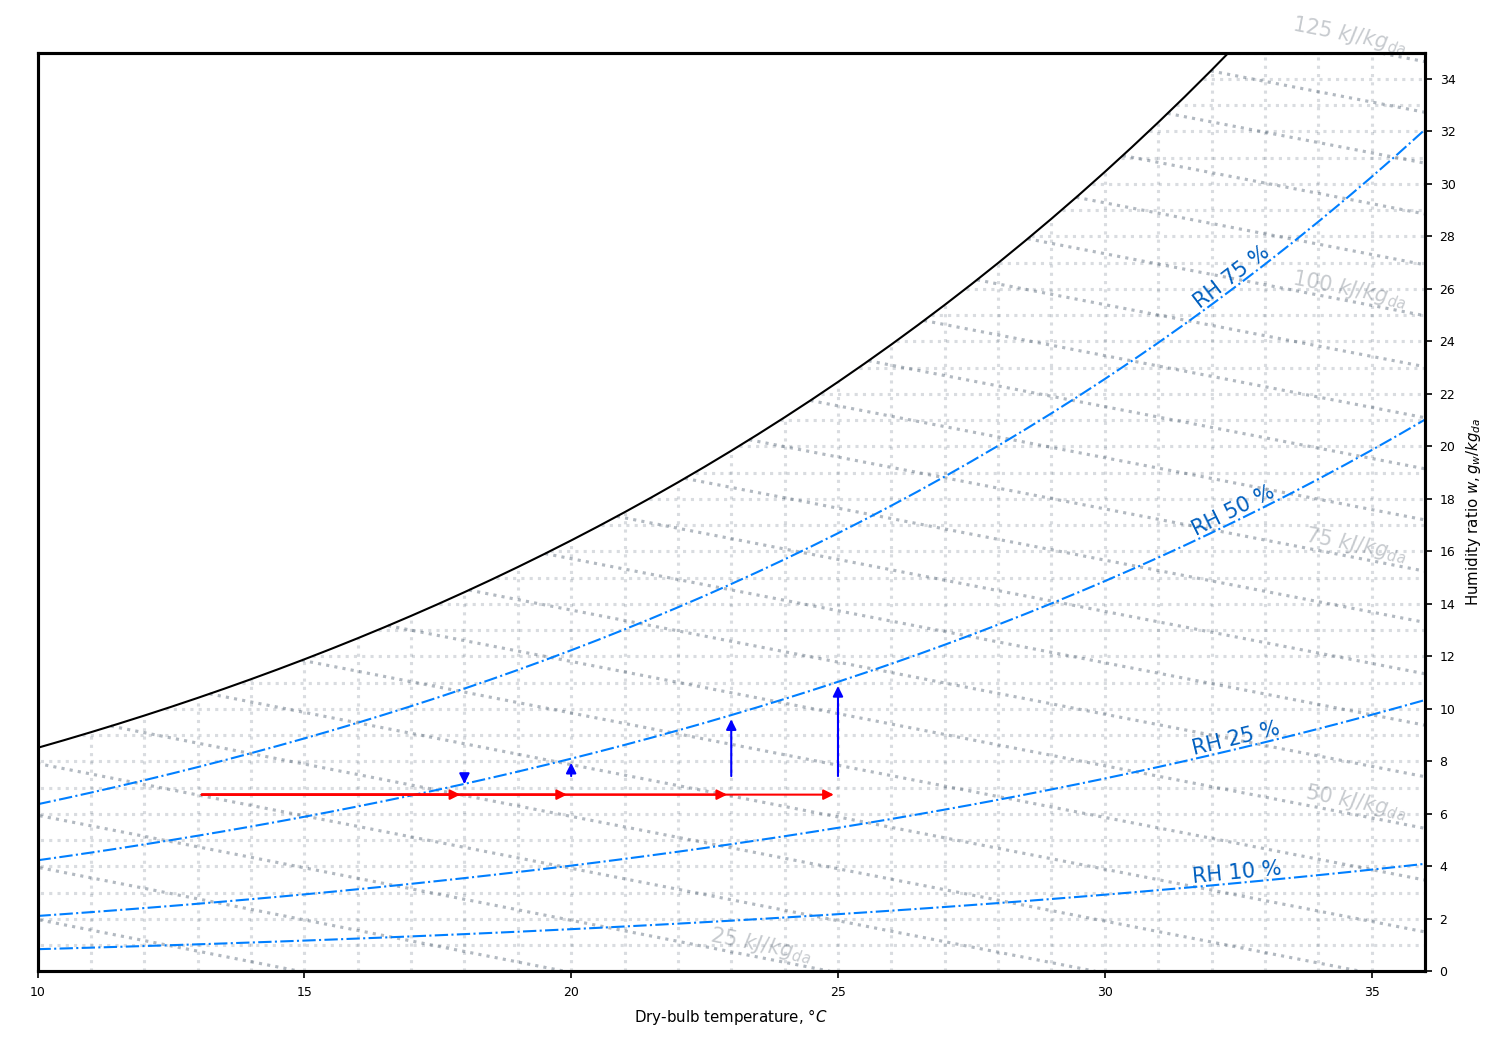
\includegraphics[width=\textwidth]{heatingcases.png}
    \caption{Example psychrometric processes under different set points for the heating scenario.}\label{fg:heat}
    \end{figure}

    Similar to the psychrometric process in the cooling case, we are expressing the heating of air in the psychrometric chart underneath. Since the majority of the heating is accomplished through furnaces and air conditioners, the outdoor air is assumed to go through a constant-humidity-ratio process as it is heated sensibly. Without additional humidifiers, the resulting RH could reach beneath 30\% (as indicated in the figure), and potentially lead risks of the occupants’ wellbeing. Even when considering additional humidifiers, the energy that needs to be added to the air can also be characterized as additional energy demands (as marked by the red arrows in illustration we created. %Check this paragraph

    It is, therefore, crucial to provide an estimation of the overall energy demand necessary to deliver air that is warm enough for all-air systems or radiant system, and additionally air that is moist enough to avoid strain on the respiratory system of the occupants. We believe it is crucial to highlight the energy savings in both the cooling and the heating condition when considering expanded set points. Using the psychrometric-driven approach, we are hoping to conduct both spatial and statistical analysis on the resulting RH and energy demand across continental US with the NOAA data we collected. %Check this paragraph

    %Energy difference - ratio of dry vs. latent.
    Beyond the first hypothesis, we would also like to assume an alternative scenario where humidifiers are used to ensure a satisfying humidity condition. This is expressed with the blue arrows in Figure~\ref{fg:heat}. With the added humidity into the air, the added latent load for all-air systems can be considered as the load that is not often characterized in the existing literature. Without specifying the systems that are used in this process and their respective efficiencies, analyzing only the requried latent load that needs to be added to the moist air through humidifier can help us understand the extra energy that is necessary when attempting to achieve desirable RH condition for the indoor environment across different set points. 

    The RH difference will be compared with the mean value. The energy saving percentage will be compared with daily average? monthly average? heating season? 


    \subsection{Data Collection and Processing}
        As we are interested in understanding the potential energy savings and RH improvement across continental US, we need the weather data collected from major cities across the continent with resolution smaller than every hour. The ISD-lite dataset made available by NOAA (National Oceanographic Association of America) provides air temperature, relative humidity and geographic location at weather stations across major city centers and airports across continental US. This data is publicly available on NOAA’s ftp server. We downloaded a total of 13,800 files for the monitored weather in 2018 for the purpose of this analysis. Since the climate zones, as we are plotting in Figure~\ref{fg:stations}. 

\begin{figure}[h!]
\centering
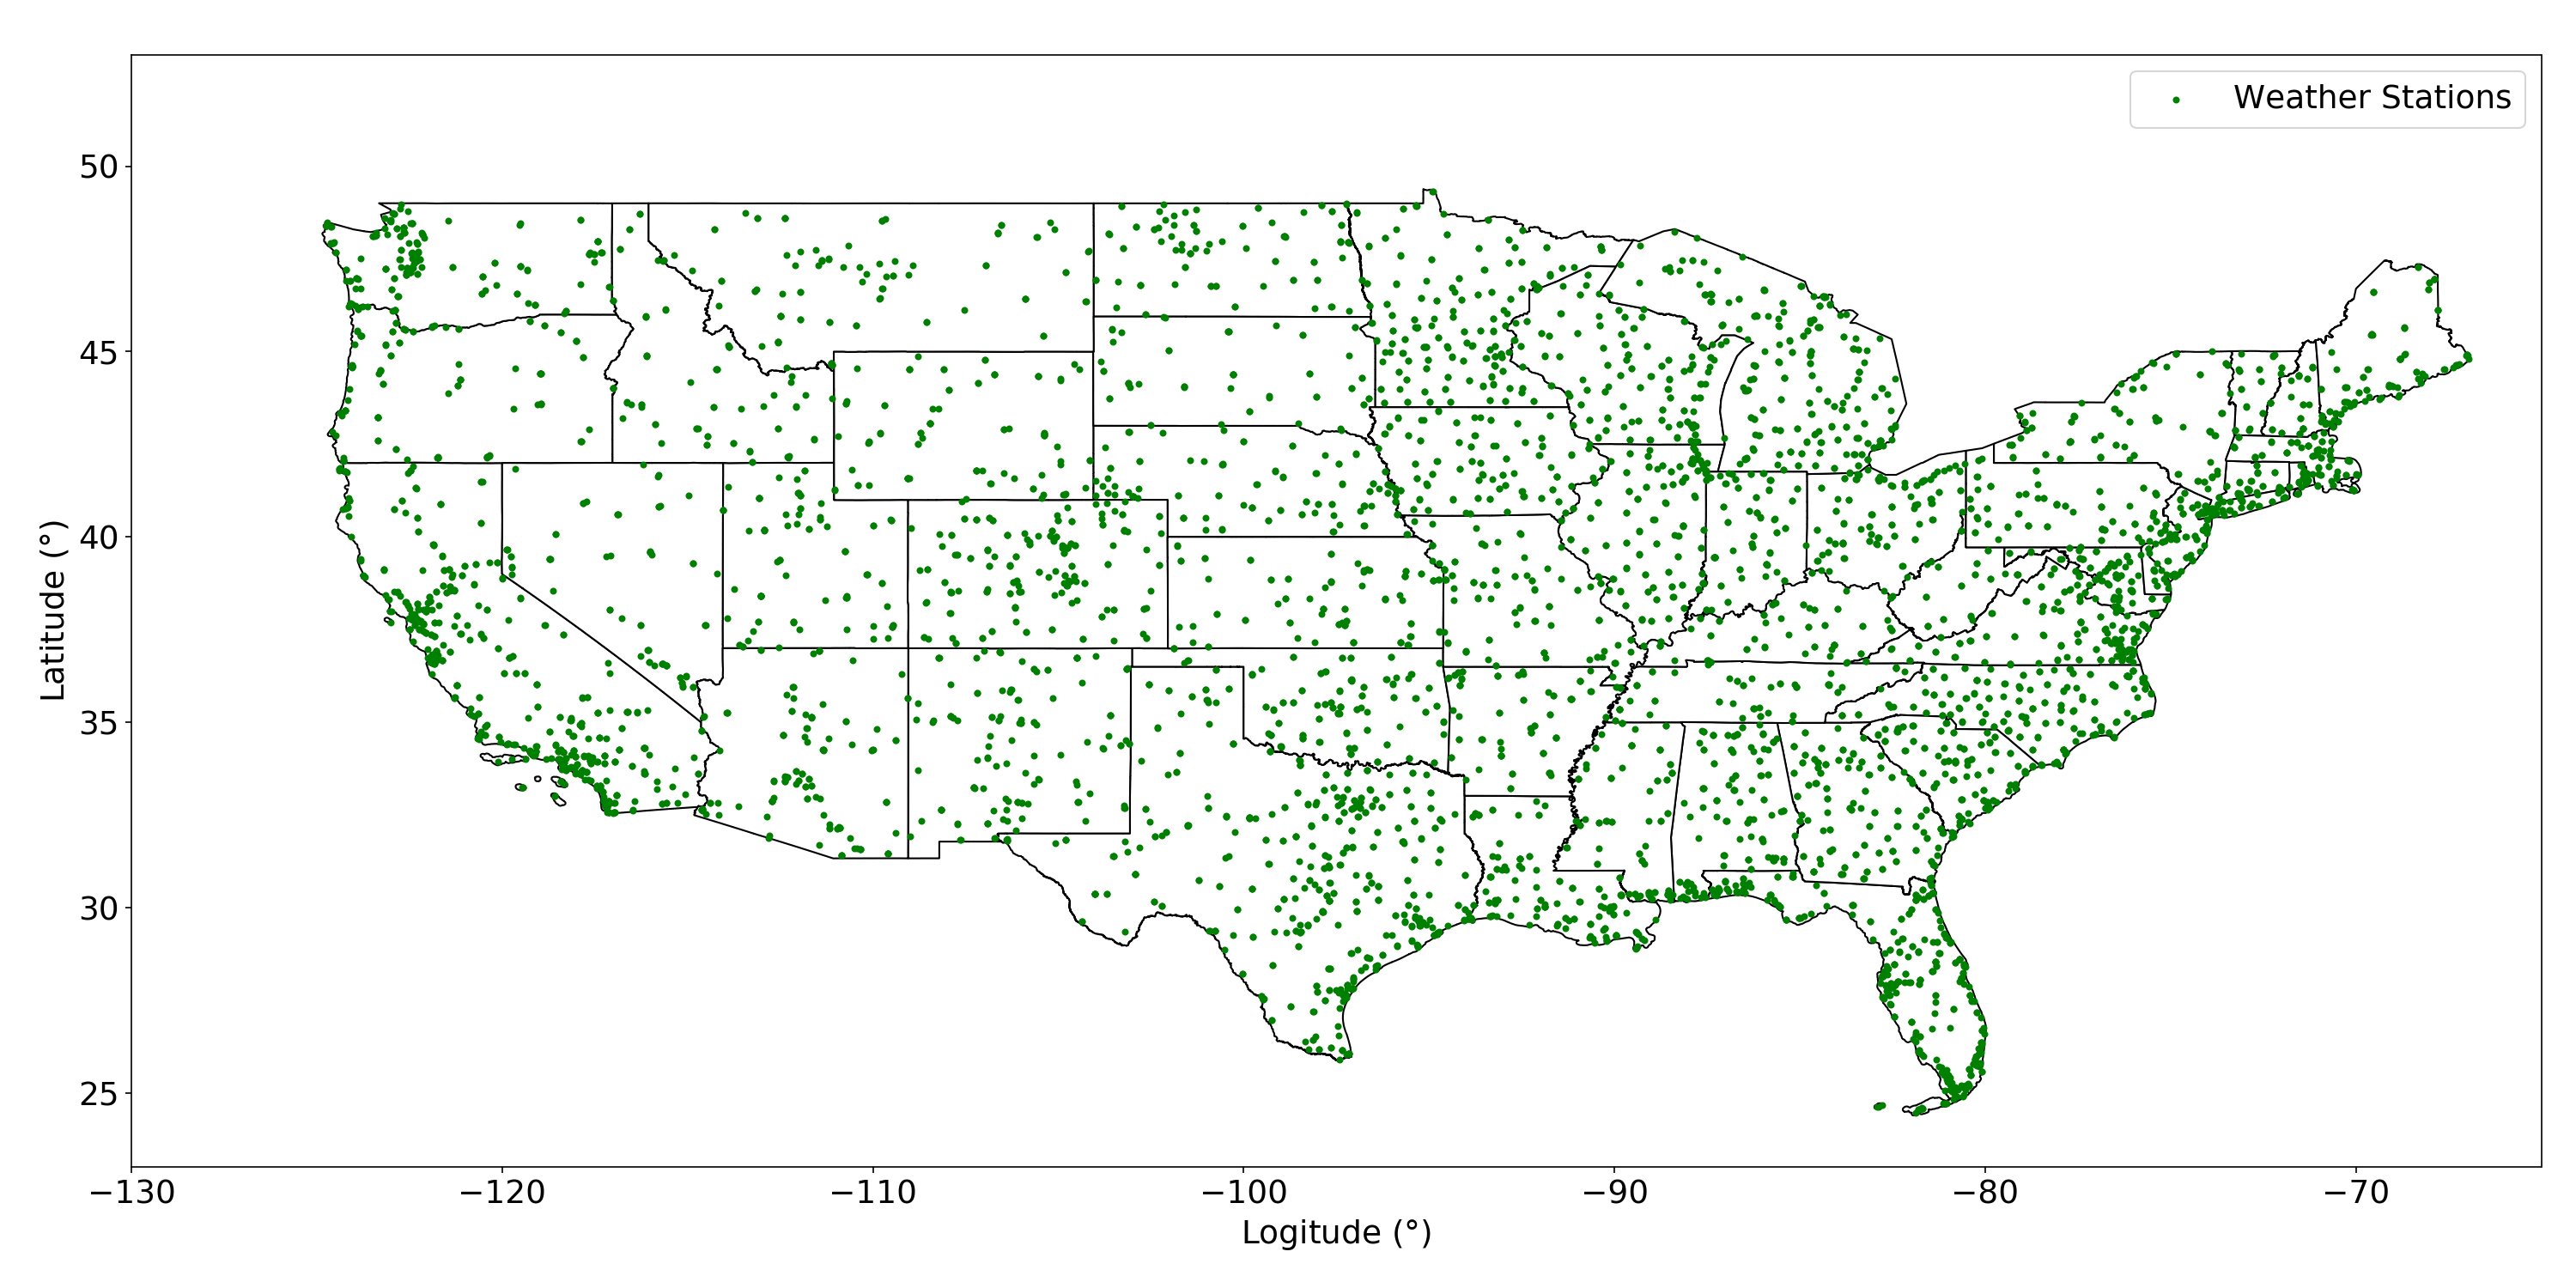
\includegraphics[width=\textwidth]{stations.png}
\caption{Locations of climate station files clipped to the USGS geometry in NOAA ISD-lite, 2017.}\label{fg:stations}
\end{figure}

Upon scraping the NOAA ftp server for the 2018 weather files, we used the pandas data frame library in Python to clean up and regroup the files into time-stamped weather data, and re-sampled on an hourly rate. We also used the CoolProps library to calculate the enthalpy of moist air at different states, and appended the resulting hourly enthalpy states. The resulting weather files will therefore have the air temperature, relative humidity, specific enthalpy for 8760 hours in 2018 across all the stations. We are plotting an example of the data collected in one of the weather stations in Figure~\ref{fg:sampleh}.


\begin{figure}
\centering
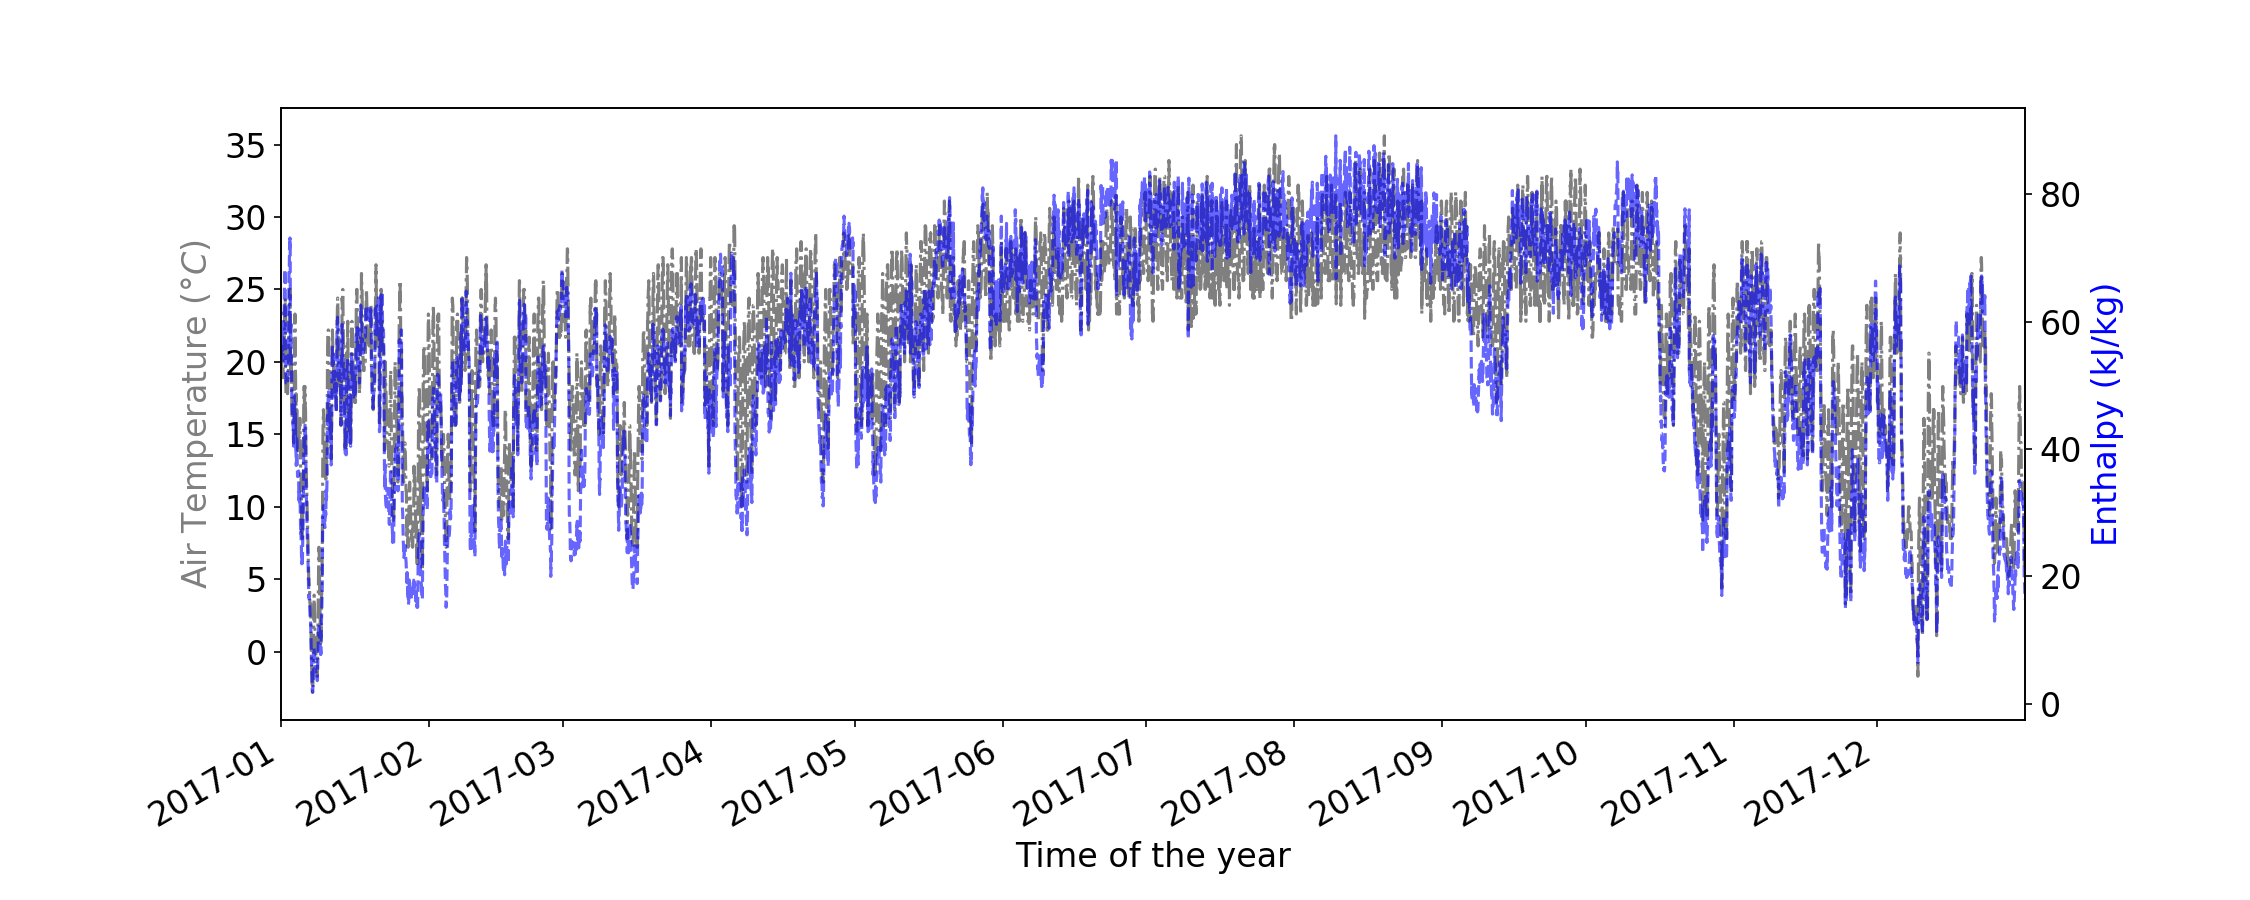
\includegraphics[width=\textwidth]{tbd_h.png}
\caption{ Processed Outdoor Dry-bulb temperature against outdoor specific enthalpy for the weather station in Station ID.}\label{fg:sampleh}
\end{figure}


We will primarily divide our analysis into two parts. The first part focuses on the energy savings of the cooling scenario and the RH improvements for the average heating/cooling condition for the weather stations. 

The second part will examine the entire time series of weather data across different climate zones. 

\section{Results}
    \subsection{Heating scenario and resulting RHs}
    Heating scenario. Resulting plot of heat map. 
%TODO Make a diagram of how the data is processed. Flow chart? 
\subsubsection{Relative Humidity}
	Assuming no additional humidifiers, the resulting relative humidity inside an average household can be easily modelled by assuming constant humidity ratio heating through assumed processes as we have illustrated in the methodology. We can estimate the relative humidity of the corresponding area on continental United States, or as shown in Figure~\ref{fg:RHmap}. 

	\begin{figure}[h!]
	\centering
	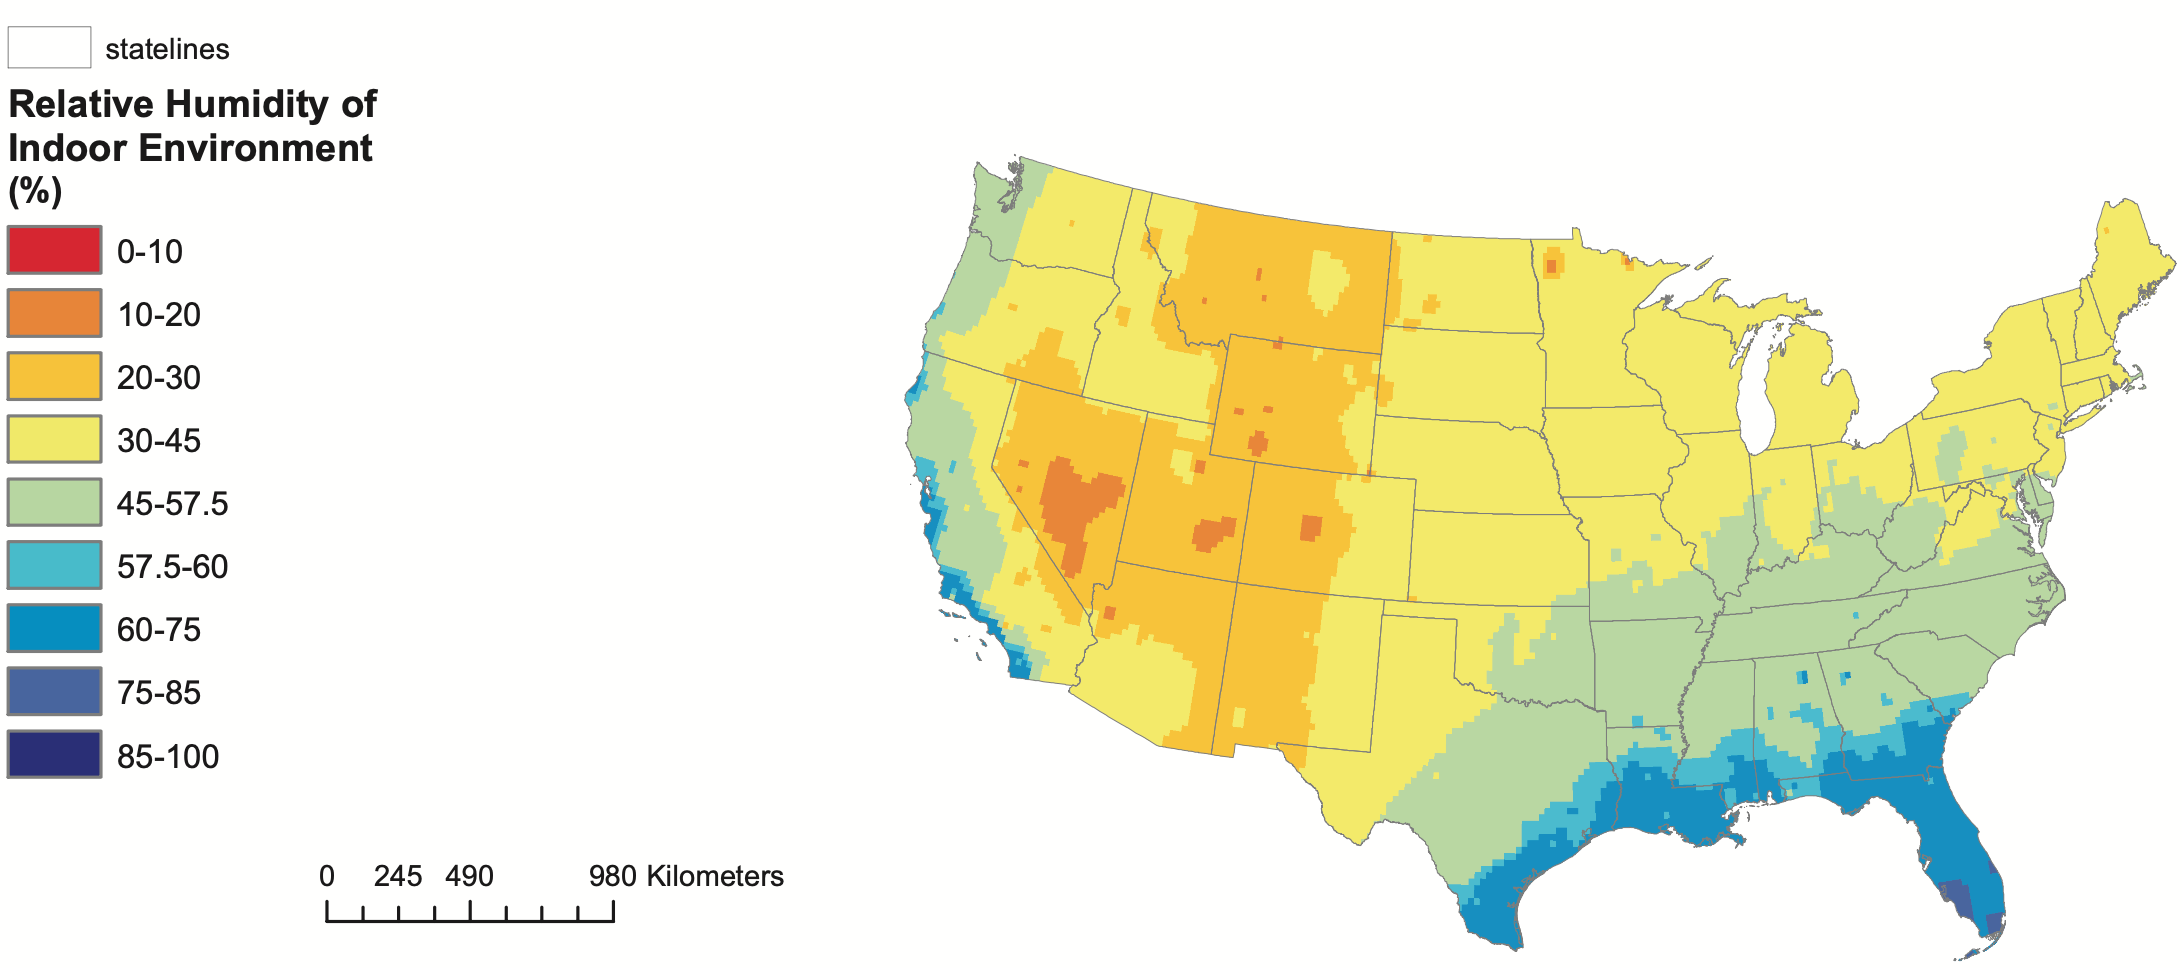
\includegraphics[width=0.7\textwidth]{heat62.png}\\
	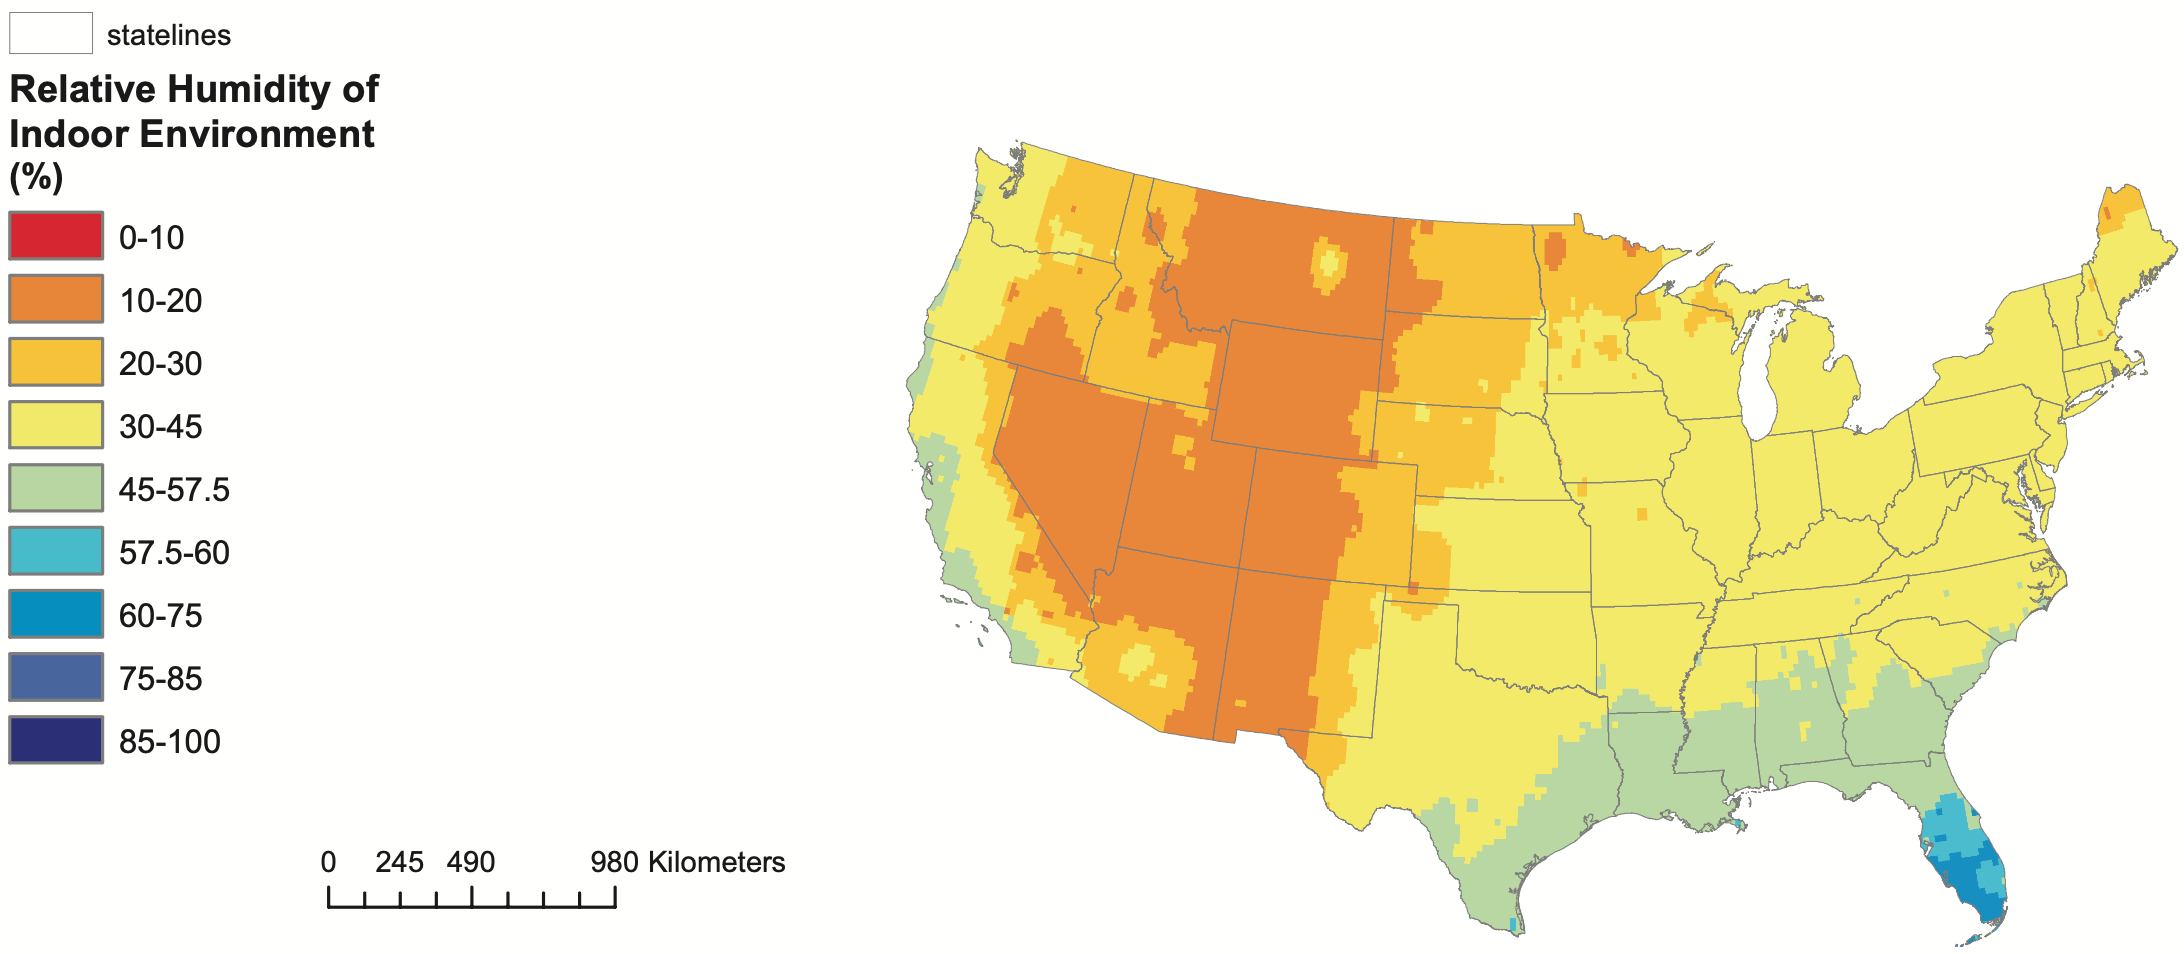
\includegraphics[width=0.7\textwidth]{heat68.png}\\
	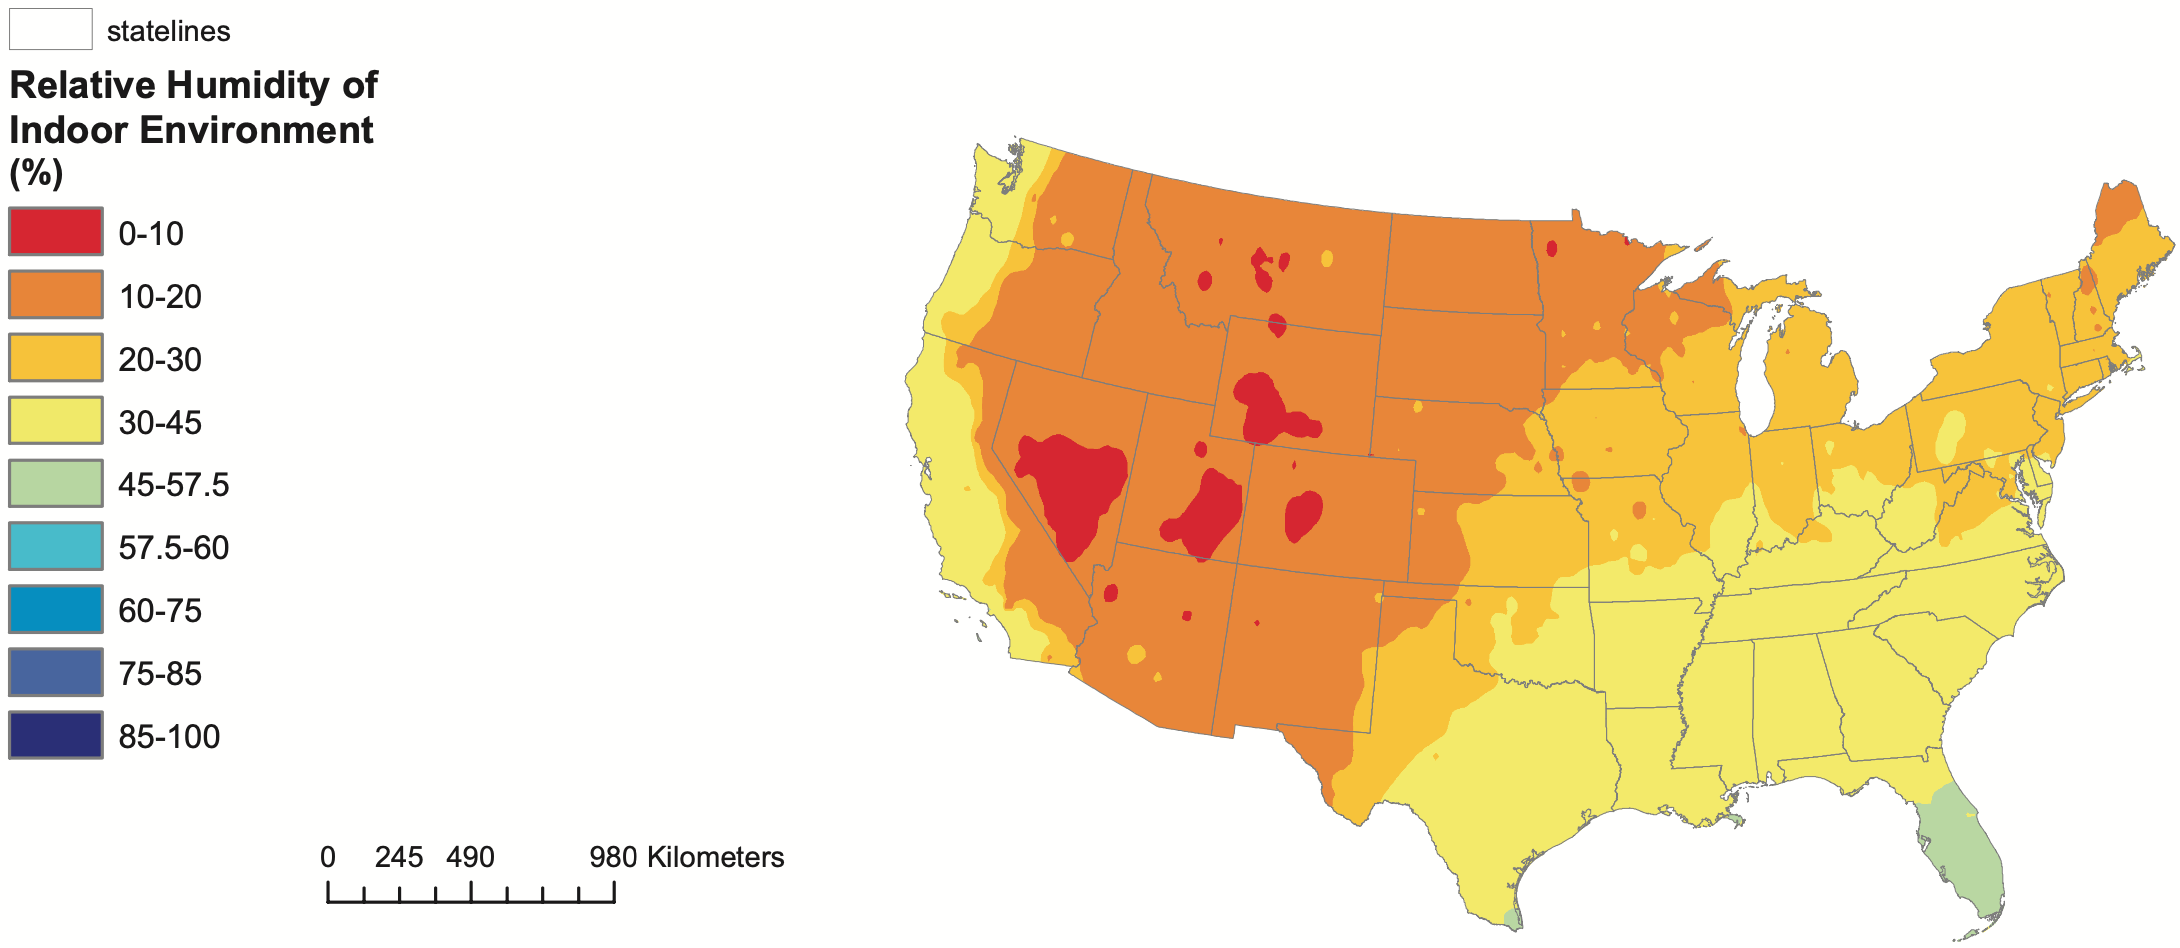
\includegraphics[width=0.7\textwidth]{heat74.png}\\
	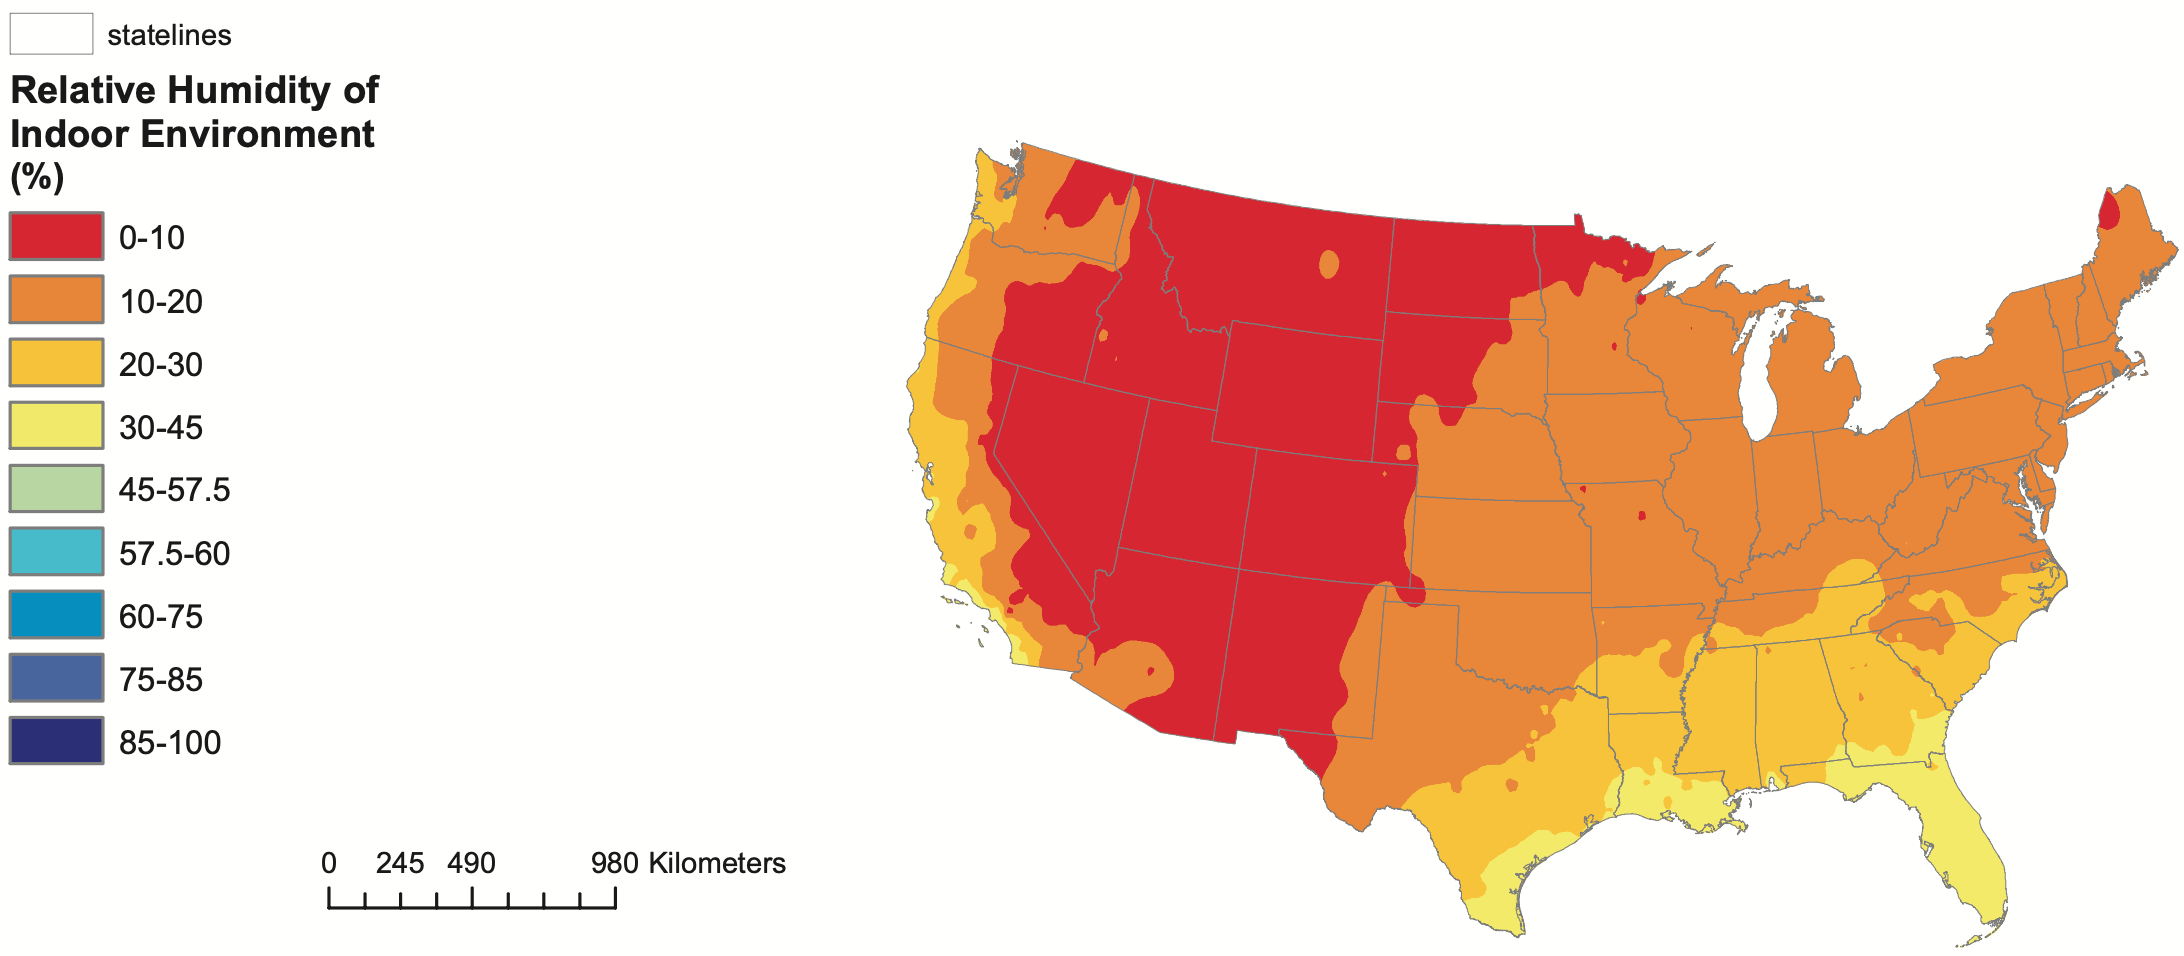
\includegraphics[width=0.7\textwidth]{heat80.png}
	\caption{Relative Humidity map generated for four different set points in Continental US.}\label{fg:RHmap}
	\end{figure}

	As we are only assuming the air undergoes a constant humidity ratio process of being sensibly heated up, the resulting heat map shown in Figure~\ref{fg:RHmap} is a very good indicator on how the set points may affect the relative humidity of an indoor environment without additional humidifiers added to the systems. From top to bottom, we plot the resulting relative humidity distribution for the four set points we selected previously, with the lowest heating set point (18 $\degree C$) on the top, and the highest set point temperature (26.7 $\degree C$) at the bottom. For the highest set point (80 $\degree F$, or 26.7 $\degree C$), an air-based system will obviously require additional humidifiers. This applies to the entire continental US, as the majority of country will result in an indoor humidity lower than the ASHARE mandate of 30\%. Using a lower set point temperature, in this case 20 and 23.3 $\degree C$, clearly improves the relative humidity of the indoor environment. However, there is still approximately 63.5\% of the entire country (weighted by area) that may have a relative humidity lower than the ASHRAE recommendation of 30\% for the set point of 23.3 $\degree C$. This number is lower for the set point of 20 $\degree C$ at 42.1\%, but still significant enough to raise concerns. Using a set point of 18 $\degree C$ appears to eliminate most of the humidification requirements, particularly for the midwest area in the continental US. However, the resulting RH distribution in the southeast area appears to create excessively high RH levels, which may suggest a higher set point for all-air system is more desirable.

	We also want to point out that the set point temperature here is not the equivalent of the supply air temperature. The set point temperature we are using is merely an indicator of the minimum amount of energy that needs to be delivered to ensure the state of the air. This psychrometric approach should not be confused with the actual energy demand of buildings, which will likely be much higher due to the infiltration, presence of the occupants, and other potential disturbances of an ideal indoor environment. 

\subsubsection{Energy Savings}
	To address the low RH problem in the residential homes when using all-air systems, an ideal solution will be to use humidifiers - which could help us investigate the energy implications when additional humidifiers are needed. Conversely speaking, this could also be considered energy savings potential from radiant systems, where a lower set point temperature is made possible at a higher relative humidity. 

	To provide a better quantitative comparison of the energy savings potentials, we will be comparing our results through the CDD and EDD calculations of the data files from selected major cities across all climate zones.

	\begin{figure}[h!]
	\centering
	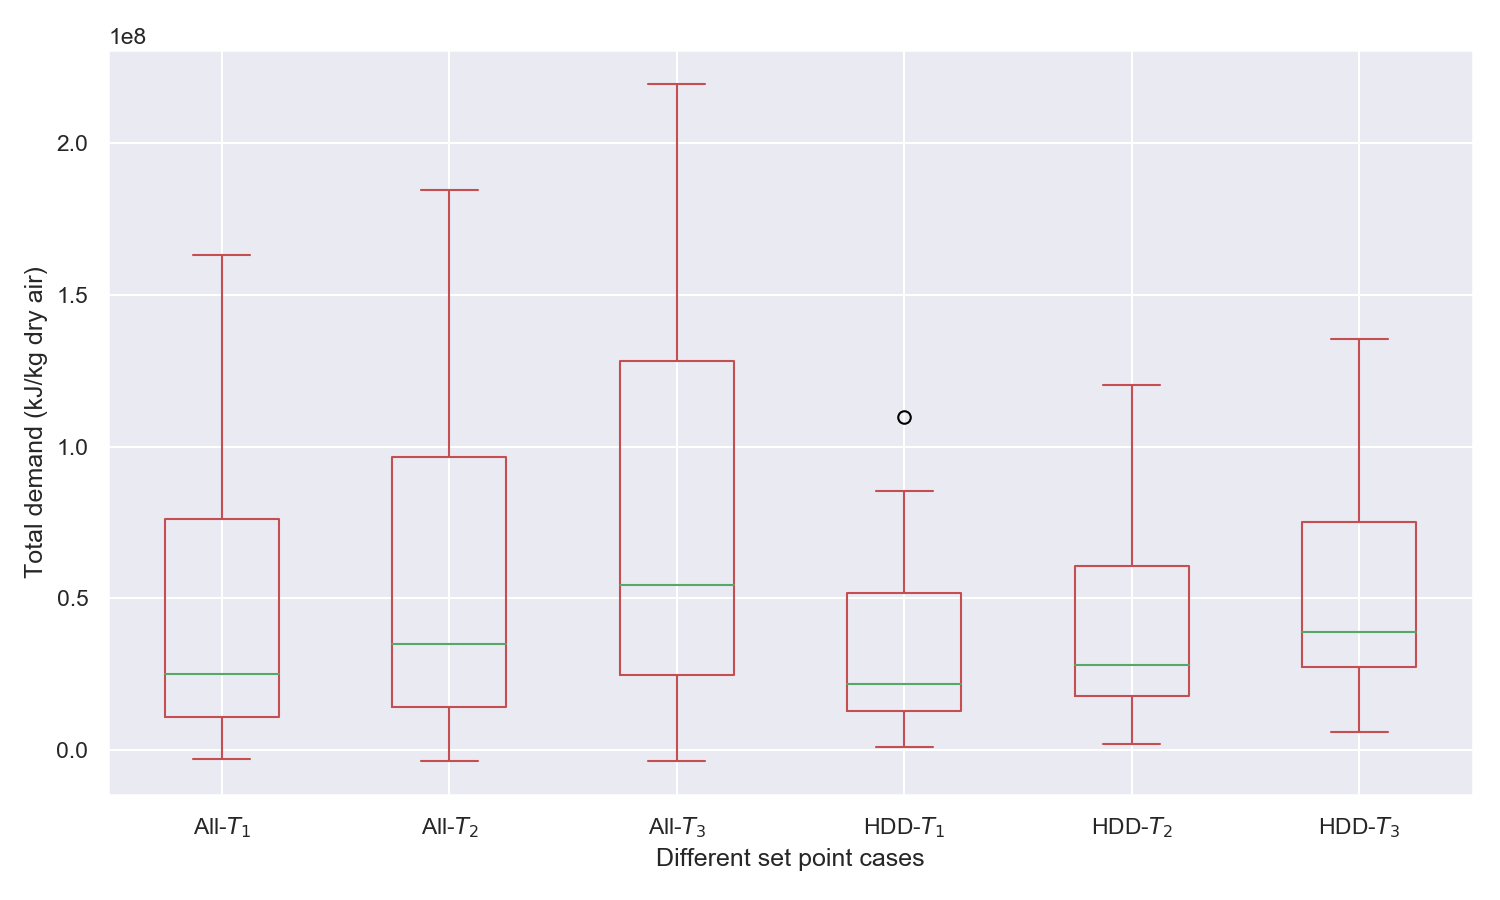
\includegraphics[width=0.8\textwidth]{boxheat.png}
	\caption{Box plot comparing the total energy demand from psychrometric analysis over dry-bulb only analysis}\label{fg:heatall}
	\end{figure}

	To visualize the overall energy demand change, we are plotting the overall demand and the corresponding heating degree day (sensible) demand in Figure~\ref{fg:heatall}. The influence on energy demand from the need to humidify the air is obvious, as the total demand increases when the set point increases from $T_1$ to $T_2$. However, the overall separation bewteen the different weather stations appears to widen. To better understand how this is affecting the different major cities through different climates, we have also plotted Figure~\ref{fg:heatcities} to illustrate how the additional energy necessray to humidify the air changes between different cities.

	\begin{figure}[h!]
	\centering
	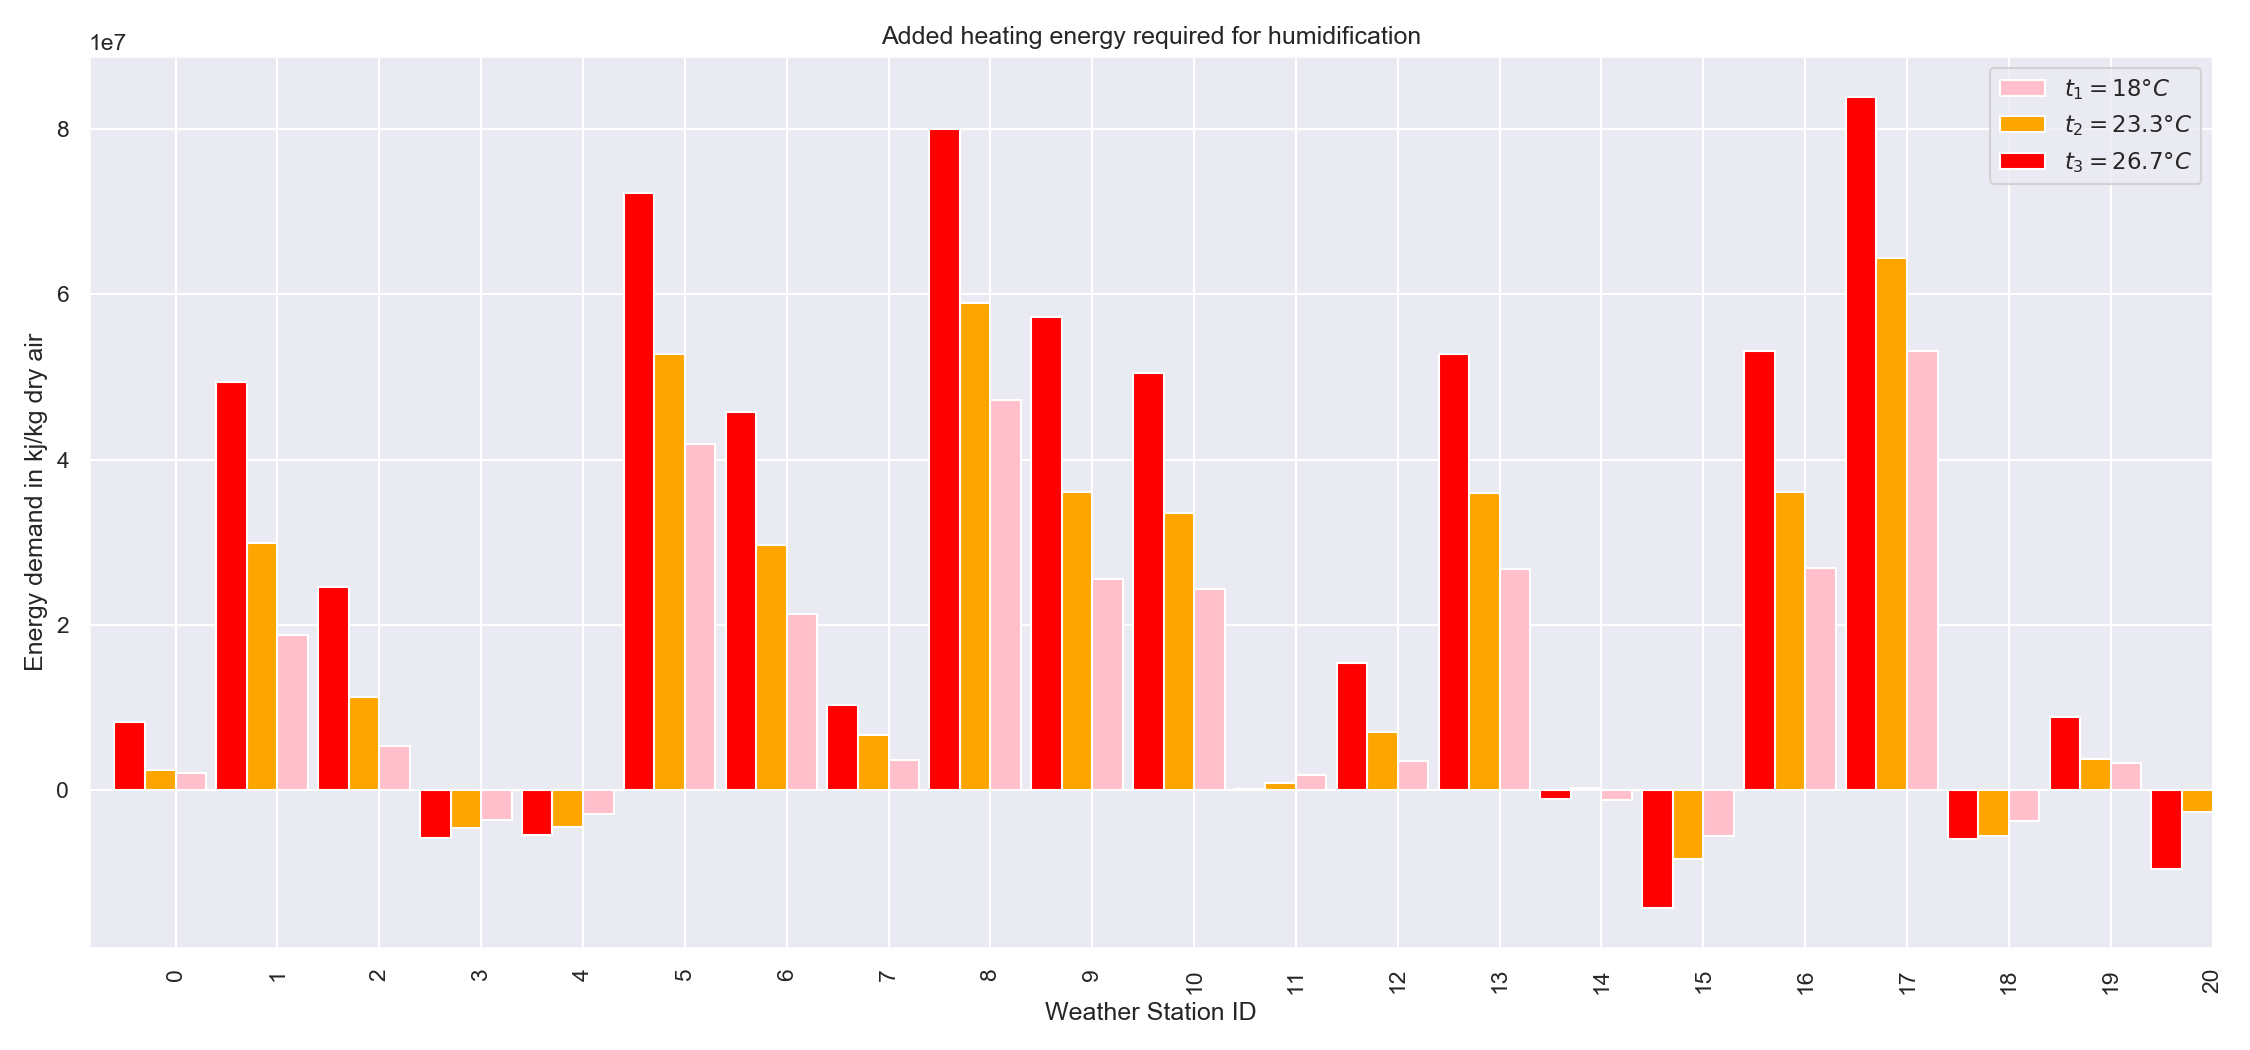
\includegraphics[width=0.8\textwidth]{heatsave.png}
	\caption{Box plot comparing the total energy demand from psychrometric analysis over dry-bulb only analysis}\label{fg:heatcities}
	\end{figure}

	According to Figure~\ref{fg:heatcities}, 71.4\% of all the stations we harvest data for will require energy to achieve at least 50\% humidity for the indoor environment. For cities in colder environments, the energy required to humidify the air could increase significantly when the set points are higher, ranging from 60\%  (Station ID=8) to up to 95\% (Station ID = 6). As our interests are primarily psychrometric-based, it is important to note that this does not reflect how different systems consumes and delivers said states of humid air, only how much energy needs to be delivered from the systems to the outdoor air to maintain a satisfying indoor environment. 
    \subsection{Cooling scenario and resulting Energy Savings}
    %Cooling Energy Savings Potential
The energy savings that can be achieved through improved set points is primarily from the variations of enthalpy differences, which represents the total energy that needs to be delivered by the HVAC systems. This can be further compared through the comparison of the differences between the cooling degree days calculated through the weather files. The total energy demand (sensible and latent) comapred with the sensible load only will not only provide us an estimation of the breakdown of the total energy demand, but also how these numbers vary by states and/or climate zones. 

The results we obtained for the by-state comparison are listed as the following box plot.


The results we obtained for the 
\section{Discussions and Conclusions}
    \subsection{Relative Humidity improvements}
    The relative humidity improvements that we identified carries some very interesting weight in furthering our evaluation of different system types. Traditionally, radiant cooling systems are only used when the relative humidity and dew point temperatures of an environment does not pose a threat to condense, otherwise the system will need to be carefully engineered to avoid condensation problems. Radiant heating systems (primarily radiators and radiant floor heating) primarily occurs in larger multi-family or high-rise residential buildings when district-level heating is possible. Although radiant heating systems were repeatedly suggested by researchers to provide better thermal comfort in comparison to air-based heating systems, some recent studies have argued against it. This improvement in relative humidity due to reduced set point temperature in radiant systems has, insofar, yet to be a major topic in the field of building engineering.

There are a number of possible answers to its absence. The first being many of the existing radiant heating systems uses 75 $\degree F$ (23.89 $\degree C$) air temperature as the feedback control variable of radiant systems. This dry-bulb air temperature is meant to ensure the occupant comfort situation inside the conditioned space. However, radiant systems are fundamentally responsible for providing a satisfying radiant environment that ensures satisfiable heat dissipation of the occupants despite the heating loads from the envelope and other miscelleneous equipments. Radiant systems are not meant to serve as heat exchangers that heats up the indoor air and maintain it at 75 $\degree F$. The authors have recently done some research with respect to the possibility of separating the radiant sensing from the air temperature sensing such that the two modes of heat exchange can be viewed separately, but there has yet to be adequate research or technology in the market that allows such separation. Up to now, it is still very common to equate thermal comfort as operative temperature as measurement of globe temperature as air temperature. We believe it is important to emphasize their differences and argue for further improvements in the state-of-the-art technology in the field.

    \subsection{Extra energy savings and demands}
    %!TEX root = _all.tex

Alternatively, the energy savings that we have been able to identify for both the heating and the cooling are also of different orders of magnitude. Comparing the order of magnitude of the energy that needs to be added/removed from the air shown in Figure~\ref{fg:heatall} and ~\ref{fg:coolall}, the latent heat that needs to be removed could be up to 10 times larger than that of the humidity requires adding, which speaks to the order of magnitude of the energy demand from de-humidification processes. However, it is equally important to stress that our discussion within the scope of this paper is purely driven by the psychrometric process.

More explicitly speaking, the latent component of the heating and the cooling scenarios are fundamentally different. For the heating scenario, the latent load is the humidity that needs to be added by humidifiers to maintain satisfying level of humidity (50\% in this study). For the cooling scenario, the latent load we were comparing was obtained by separating the sensible from the total cooling demand resulting from outdoor air. Therefore, for the heating scenario, the energy that needs to be added to the air through humidifiers cannot be directly translated into energy demand. For the cooling scenario, the the differences between the latent energy are in fact the energy demands that can be reduced through selection of different set points.

However, regarding the humidity removal process,it's also important to point out that neither of the scenarios can be directly translated into energy savings as there may potentially be different systems invovled in achieving the desirable state of humid air. This allowed us to avoid focusing on a specific type of building system and its corresponding component effiiencies within the scope of this analysis. Further discussions regarding the benefits of selecting certain humidity removal technologies, such as the chilled water cooling/heating system, dual (dessicant and enthalpy) wheel or direct exchange cooling coils. 

\section{Conclusion}
%!TEX root = _all.tex
We examined the heating and cooling of the humid air across continental US and analyzed the energy savings potential that can be expected when alternative set points are used. A highlight of this study is how the heating potential is analyzed and the energy savings analyzed for better understanding of the potential energy savings of radiant systems. Beginning with pure psychrometric analysis, we use the humid air properties of the air to determine the amount of heating and cooling that is necessary to achieve a desirable state for the humid air. This analysis is independent of a specific type of air handling and a predetermined process of a given system, and is generically applicable for large-scale analysis. To do so, we used the weather data files made available by the NOAA ISD-lite project, and estimated the overall heating degree days and cooling degree days against its enthalpy degree days to further characterize the latent loads that occur for different cities in different climate zones. We obtained results that shows the energy savings potential for both the heating and the cooling scenarios across the country.

We hope the results from this study can help further investigations being directed at the latent loads in buildings that are caused by using all-air systems for both the heating and the cooling scenarios. Although we have demonstrated that there are energy savings potentials through expanding the set point temperature for the indoor environment, the scope of investigation of this paper does not extend to specific systems or components, and should therefore should not be interpreted as explicit energy savings for building systems. We hope to inspire future investigations on the cooling and heating capabilities of such systems, and observe improved system designs as a result of this study.
\bibliography{top.bib}
\end{document}